\documentclass[tikz,border=10pt]{standalone}
\usepackage{tikz}
\usetikzlibrary{arrows.meta,positioning}

\tikzset{
  card/.style={draw=blue!70!black, line width=1.2pt, rounded corners=3pt, minimum width=5.2cm, minimum height=1.0cm, align=center, fill=none},
  flow/.style={-{Stealth[length=3mm]}, line width=1.2pt, draw=black!70}
}

\begin{document}
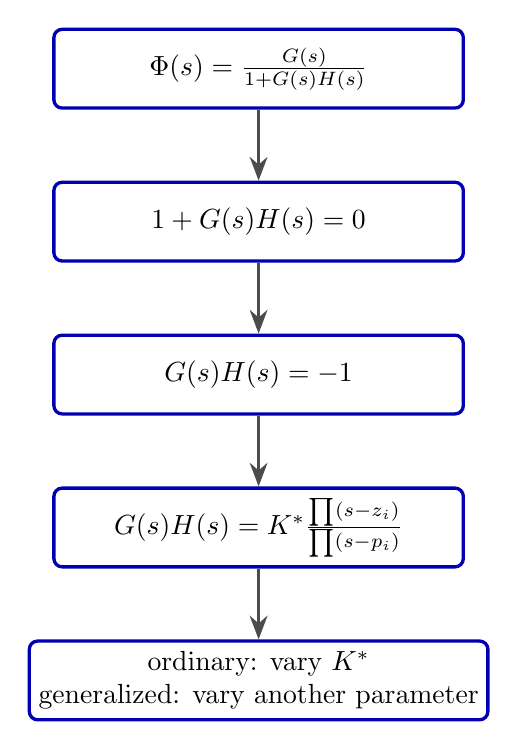
\begin{tikzpicture}[node distance=0.9cm]
  \node[card] (a) {$\Phi(s)=\frac{G(s)}{1+G(s)H(s)}$};
  \node[card, below=of a] (b) {$1+G(s)H(s)=0$};
  \node[card, below=of b] (c) {$G(s)H(s)=-1$};
  \node[card, below=of c] (d) {$G(s)H(s)=K^\ast \frac{\prod(s-z_i)}{\prod(s-p_i)}$};
  \node[card, below=of d] (e) {ordinary: vary $K^\ast$\\generalized: vary another parameter};

  \draw[flow] (a) -- (b);
  \draw[flow] (b) -- (c);
  \draw[flow] (c) -- (d);
  \draw[flow] (d) -- (e);
\end{tikzpicture}
\end{document}
